\section{Salze}
\subsection{Lösbarkeit in \acl{H2O}}
\begin{itemize}
   \item Alle Salze lösen sich in \ac{H2O}, aber unterschiedlich gut.
   \begin{itemize}
      \item Es findet eine Änderung des Aggregatzustandes statt. Dies ist ein physikalischer Vorgang.
   \end{itemize}
   \item Der Vorgang lässt sich mit mechanischer oder thermischer Energie beschleunigen.
\end{itemize}

\cVersuch{3}{Hydrations- und Gitterenergie}
\begin{description}
   \item[Aufbau und Durchführung:] Wir lösen folgende Salze in \ac{H2O} jeweils in separaten Reagenzgläsern.
   \item[Ergebnis:] \hspace{3.4cm} \includegraphics[width=5cm]{files/pst-labo/Hydraktions-pics}
\end{description}

\begin{center}
\begin{tabular}{|c|c|c|c|c|c|}
\hline \textsc{id} & \textsc{Name} & \textsc{Formel} & \textsc{löslich} & \textsc{Temperatur} & \textsc{Hydraktionenergie} \\
& & & & & \textsc{Gitterenergie}\\
\hline 1 & \aclu{NaCl} & \acsu{NaCl} & sehr gut & leicht abfallend & Hydraktionse. < Gittere. \\
\hline 2 & \aclu{CaCO3} & \acsu{CaCO3} & schlecht & keine Änderung & Hydraktionse. < Gittere. \\
\hline 3 & \aclu{CaCl2} & \acsu{CaCl2} & mittel & heftiger Anstieg & Hydraktionse. > Gittere. \\
\hline 4 & \aclu{KNO3} & \acsu{KNO3} & gut & heftiger Abfall & Hydraktionse. < Gittere. \\
\hline
\end{tabular}
\end{center}

\subsubsection{Hydratationsenergie}
Das polare Lösungsmittel \ac{H2O} zerstört das Ionengitter der Salze, indem es sich an dessen Ionen ablagert.
Diesen Vorgang nennt man eine Hydratation. Es entsteht Hydratationsenergie (Wärme wird frei).
\vspace{-0.7cm}
\begin{center}
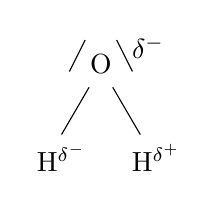
\begin{tikzpicture}[color = {black},scale = 1]
   \draw (1.1,1.8) -- (1.3,2.2);
   \draw (1.9,1.8) -- (1.7,2.2);
   \draw (1,1) -- (1.35,1.6);
   \draw (1.65,1.6) -- (2,1);
   \node[scale = 1] at (1.5,1.9) {O};
   \node[scale = 1] at (2.1,2.1) {$\delta^-$};
   \node[scale = 1] at (1,0.7) {H$^{\delta^-}$};
   \node[scale = 1] at (2.2,0.7) {H$^{\delta^+}$};
\end{tikzpicture}
\end{center}

\subsubsection{Gitterenergie}
Gitterenergie ist die Energie die das Kristallgitter aufrecht erhält. Sie muss überwunden werden. Es wird kälter.

\cVersuch{3}{Diffusion}
\begin{description}
   \item[Aufbau und Durchführung:] Mit Hilfe von Fett klebten wir etwas \ac{KMnO4} (als Salzersatz zur besseren Veranschaulichung) an einen Korken, den wir in ein Standzylinder mit \ac{H2O} legten. So war die Verbreitung des \ac{KMnO4} als violette Flüssigkeit gut zu erkennen.
   \item[Ergebnis:] Das \ac{KMnO4} verteilte sich ohne die Zuführung von mechanischer Energie langsam im Zylinder.
Diese selbstständige gleichmäßige Verteilung nennt man Diffusion.
\begin{description}
   \item[Diffusion:] Vorgang, in dessen Verlauf Teilchen in Folge ihrer Wärmebewegung auf
 unregelmäßigen zickzackförmigen Bahnen von Orten höherer Konzentration
 zu Orten niederer Konzentration gelangen. Dies führt schließlich zu einer vollständigen Vermischung.
\end{description}
\end{description}

\cVersuch{3}{Osmose}
\begin{description}
   \item[Aufbau und Durchführung:] Wir stellten je eine Blume in einen Erlenmeyerkolben gefüllt mit\begin{enumerate}\item Salzwasser\item \ac{H2O}\end{enumerate}
   \item[Ergebnis:] Bereits nach einer Stunde sah man bei der Blume im Salzwasser eine gewisse Schlaffheit.
   \begin{description}
      \item[Osmose:] Durch eine halbdurchlässige (semipermeable) Membran einseitig verlaufender Lösungsausgleich zweier gleichartiger unterschiedlich konzentrierter Lösungen, wobei sich das Lösungsmittel zum Ort hoher, zum Ort niederer Konzentration bewegt.
   \end{description}
\end{description}

\cVersuch{3}{Ausgehöhlte Kartoffel mit \acl{NaCl}}
\begin{description}
   \item[Aufbau und Durchführung:] Wir zerteilten eine Kartoffel in zwei Hälften und höhlten dies aus, anschließend streuten wir auf eine der beiden Hälften \ac{NaCl}.
   \item[Ergebnis:] Bei der Kartoffelhälfte mit \ac{NaCl} trat viel \ac{H2O} aus und diese sah leicht vertrocknet aus. Bei der Anderen war nichts der Gleichen zu beobachten.
\end{description}

\cVersuch{3}{Natriumhydroxidtabletten und Luftfeuchtigkeit}
\begin{description}
   \item[Aufbau und Durchführung:]  Wir gaben etwas \ac{NaOH} als Salzersatz auf eine Kristallisierschale.
   \item[Ergebnis:] Nach einem Tag waren die zuvor festen Natriumhydroxidtabletten aufgeweicht, und auf der Schale hatte sich Wasser angesammelt.
\end{description}

\newcounter{cVersuchSubtra}\setcounter{cVersuchSubtra}{\value{cVersuch}}\addtocounter{cVersuchSubtra}{-1}
\subsubsection{Begründung für Experiment \arabic{cVersuchSubtra} und \arabic{cVersuch}}
Viele Salze sind hygroskopisch, das heißt sie entziehen der Umwelt das \ac{H2O}.

\cVersuch{3}{Löslichkeit von \acl{NaCl} gegenüber \acl{C2H5OH}}
\begin{description}
   \item[Aufbau und Durchführung:] Wie gaben \acl{CuSO4} und \acl{C2H5OH} in ein Becherglas.
   \item[Ergebnis:] \ac{C2H5OH} ist besser in \ac{H2O} löslich als \aclu{CuSO4} ($\mathrm{\stackrel{\RM{2}}{Cu}\stackrel{\RM{2}}{SO_4}}$), \ac{CuSO4} fällt aus.
\end{description}

\cVersuch{3}{Siedepunkterhöhung}
\begin{description}
   \item[Aufbau und Durchführung:] Auf einen Dreifuß stellten wir ein Becherglas, darin wurde \ac{H2O} zum Sieden gebracht und anschließend \ac{NaCl} dazugegeben.
   \item[Ergebnis:] Knallen, Schäumen und ein Temperaturanstieg, \begin{description}\item[Erhöhung des Siedepunkts:] Erhöhung der Temperatur, bei der eine Substanz vom flüssigen in den gasförmigen Zustand übergeht.\end{description}
   Beim Sieden verdunstet \ac{H2O}. Die Salzlösung wird konzentriert. Salz müsste schließlich ausfallen. Das System, versucht diesem Phänomen auszuweichen. Es kommt zum Temperaturanstieg um eine bessere Lösbarkeit zu erreichen.
\end{description}
\begin{center}
   \includegraphics[width=2cm]{files/pst-labo/Siedepunkter-pics}
\end{center}


\cVersuch{3}{Gefrierpunkterniedrigung}
\begin{description}
   \item[Aufbau und Durchführung:] Wir gaben ein paar Eiswürfel in ein Becherglas und streuten \ac{NaCl} darauf. Das Eis fing an, flüssig zu werden. Wir stellten das Glas auf eine nasse Fläche und ein Reagenzglas mit \ac{H2O} in das Becherglas.
   \item[Ergebnis:] Nach wenigen Minuten war das Becherglas auf dem Tisch fest gefroren. Das \ac{H2O} im Reagenzglas, dass in der \ac{NaCl} Lösung stand, war ebenfalls gefroren.\\
   Damit bewiesen wir, dass Salzlösungen nicht wie \ac{H2O} bei 0°C gefrieren.\\
Es fand eine Gefrierpunkterniedrigung (Herabsetzung der Temperatur bei dem ein Stoff vom flüssigen in den festen Zustand übergeht) statt.
\end{description}

\cVersuch{2}{Erhitzen von \acl{CuSO4.5H2O}}
\begin{description}
   \item[Aufbau und Durchführung:] Wir erhitzten \ac{CuSO4.5H2O}
   \item[Ergebnis:] Bei leichtem Erhitzen entstand weißes Anhydrit (ohne Wasser, wurde ausgetrieben). Nach starkem Erhitzen entstand Säuregas.
\end{description}

\subsection{Weitere Salzbildungsarten}
\cVersuch{3}{\acl{12} in \acl{H2CO3}}
\begin{description}
   \item[Aufbau und Durchführung:] Wir gaben \ac{12} und \ac{H2CO3} in ein Reagenzglas.
   \item[Ergebnis:] Es zischte und es entstand Wasserstoff, den wir mit der Knallgasprobe nachwiesen. \\
   \ce{Mg + 2HCl -> MgCl2 + H2} \\
   \ce{Mg + 2H^+ + 2Cl^- <=> Mg^2+ + 2Cl^- + H2} \\
   unedles Metall + Säure \ce{->} Salz + \acl{H2}
\end{description}

\begin{center}
\includegraphics[width=2cm]{files/pst-labo/CuOundH2SO4-pics}
\end{center}


\cVersuch{3}{Kupfer(II)-oxid in \acl{H2SO4}}
\begin{description}
   \item[Aufbau und Durchführung:] Wir gaben \ac{CuO} in ein Reagenzglas und gaben verdünnte \ac{H2SO4} dazu.
   \item[Ergebnis:] Die Flüssigkeit verfärbte sich von grau-schwarz nach grün. Salz viel aus. \\
   \ce{CuO + H2SO4 -> CuSO4 + H2O} \\
   $\mathrm{\Delta}$EN 1,9; 3,5 \\
   $\mathrm{\Delta}$EN = 1,6 < 1,7 $\rightarrow$ polare Atombindung \\
   \ce{CuO + 2H^+ + SO4^2- <=> Cu^2+ + SO4^2- + H2O} \\
   Metalloxide + Säure \ce{->} Salz + \acl{H2O}
\end{description}

\cVersuch{3}{\acl{30} und \acl{16}}
\begin{description}
   \item[Aufbau und Durchführung:] Wir mischten solides \ac{30} und \ac{16}, und hielten ein glühendes Metall hinein.
   \item[Ergebnis:] Das Gemisch entzündete sich mit einer grünen Flamme. Es blieb nur Salz, das wie Asche aussah zurück. \\
   \ce{Zn + S -> ZnS} \\
   Metall + Nichtmetall \ce{->} Salz
\end{description}

\cVersuch{3}{Kochsalzlösung in Silbernitratlösung}
\begin{description}
   \item[Aufbau und Durchführung:] Wir gaben Silbernitratlösung und Kochsalzlösung in ein Becherglas.
   \item[Ergebnis:] Es viel ein weißes Salz aus.
   \begin{align*}
      \cee{NaCl \aggre{l} + AgNO3 \aggre{l} &-> NaNO3 + AgCl \\
      Na^+ + Cl^- + Ag^+ + NO3^- &<=> Na^+ + NO3^- + AgCl v}
   \end{align*}
   leicht lösliches Salz + leicht lösliches Salz \ce{->} leicht lösliches Salz + schwer lösliches Salz
\end{description}

\cVersuch{3}{\acl{NaCl} in \acl{H2SO4}}
\begin{description}
   \item[Aufbau und Durchführung:] Wir gaben \ac{H2SO4} in einem Becherglas auf \ac{NaCl}.
   \item[Ergebnis:] Es begann zu rauchen und roch charakteristisch stechend. \\
   \ce{2NaCl \aggre{s} + \textit{c}\; H2SO4 -> Na2SO4 \aggre{s} + 2HCl \aggre{g}} \\
   Die stärkere Säure verdrängt die schwächere aus ihren Salzen. \\
   \ce{2NaCl + 2H^+ + SO4^2- <=> Na2SO4 + 2HCl}
\end{description}

\cVersuch{2}{\acl{13} und \acl{Br2}}
\begin{description}
   \item[Aufbau und Durchführung:] Wir gaben \ac{13} zusammen mit \ac{Br2} in einen Standzylinder, dieser stand unter einem Abzug.
   \item[Ergebnis:] Als das \ac{Br2} mit dem \ac{13} in Berührung kam, fing es an rot zu leuchten. Es war eine Rauchentwicklung zu erkennen und der Geruch war mit \ac{Cl2} vergleichbar.
\end{description}

\subsection{Definition}
Salze sind Stoffe, die in wässriger Lösung oder in der Schmelze in positiv geladene Metallionen und negativ geladene Säurerestionen zerfallen (Ionensubstanzen).

\begin{list}{}{}
   \item[Ausnahme:] \ac{NH4+} kann ein Metallion ersetzen.
\end{list}
